\section{内扩散对复合反应选择性的影响}


\begin{frame}
    \frametitle{平行反应}

    考察下列平行反应，B为目的产物：
    \[
        \ch{A -> B} \qquad r_\mathrm{B} = k_1c_\mathrm{A}^ \alpha \qquad \alpha>0
    \]
    \[
        \ch{A -> D} \qquad r_\mathrm{D} = k_2c_\mathrm{A}^ \beta \qquad \beta>0
    \]
    内扩散无影响时的选择性为：
    \[
        S^{\prime}=\frac{\mathscr{R}_{\mathrm{B}}}{(-\mathscr{R}_{\mathrm{A}})}=\frac{r_{\mathrm{B}}}{r_{\mathrm{B}}+r_{\mathrm{D}}}=\frac{k_{1} c_{\mathrm{AS}}^{\alpha}}{k_{1} c_{\mathrm{AS}}^{\alpha}+k_{2} c_{\mathrm{AS}}^{\beta}}=\frac{1}{1+\frac{k_{2}}{k_{1}} c_{\mathrm{AS}}^{\beta-\alpha}} 
    \]
    内扩散有影响时的选择性为：
    \[
        S=\frac{1}{1+\frac{k_{2}}{k_{1}}\left\langle c_{\mathrm{A}}\right\rangle^{\beta-\alpha}}
    \]

\end{frame}


\begin{frame}
    \frametitle{平行反应}

    显然，$c_{\mathrm{AS}} > \left\langle c_{\mathrm{A}}\right\rangle$，$S$与$S'$的大小就看两个反应的反应级数之差。
    \[
        \alpha=\beta \text { 时, } \quad S^{\prime}=S
    \]
    \[
        \alpha>\beta \text { 时, } \quad S<S^{\prime}
    \]
    \[
        \alpha<\beta \text { 时, } \quad S>S^{\prime}
    \] 
    \begin{itemize}
        \item 当两反应的反应级数相等时，内扩散对反应选择性无影响；
        \item 主反应的反应级数大于副反应时，内扩散使反应选择性降低；
        \item 主反应的反应级数小于副反应时，则内扩散会使反应选择性增加。
    \end{itemize}

\end{frame}


\begin{frame}
    \frametitle{连串反应}
    考察一级不可逆连串反应：
    \[
        \ce{A ->[k_1] B ->[k_2] D}
    \]
    内扩散有影响时：
    \[
        S=\frac{\mathscr{R}_{\mathrm{B}}^{*}}{\mathscr{R}_{\mathrm{A}}^{*}}=\frac{1}{1+\sqrt{k_{2} / k_{1}}}-\sqrt{\frac{k_{2}}{k_{1}}} \times \frac{c_{\mathrm{BS}}}{c_{\mathrm{AS}}} 
    \]
    内扩散无影响时：
    \[
        S^{\prime}=\frac{\mathscr{R}_{\mathrm{B}}}{(-\mathscr{R}_{\mathrm{A}})}=\frac{k_{1} c_{\mathrm{AS}}-k_{2} c_{\mathrm{BS}}}{k_{1} c_{\mathrm{AS}}}=1-\frac{k_{2}}{k_{1}} \times \frac{c_{\mathrm{BS}}}{c_{\mathrm{AS}}}
    \]
    比较两式可知，由于内扩散的影响，使反应的瞬时选择性降低。

\end{frame}


\begin{frame}
    \frametitle{连串反应}

        \begin{minipage}{0.45\linewidth}
            \begin{itemize}
                \item 内扩散的存在，使目的产物B的收率降低
                \item 内扩散的影响越严重，收率降低得越多
                \item 必须采取措施使内扩散对过程的影响减到最小
            \end{itemize}
        \end{minipage}\hfill
        \begin{minipage}{0.53\linewidth}
            \begin{figure}[htpb]
                \centering
                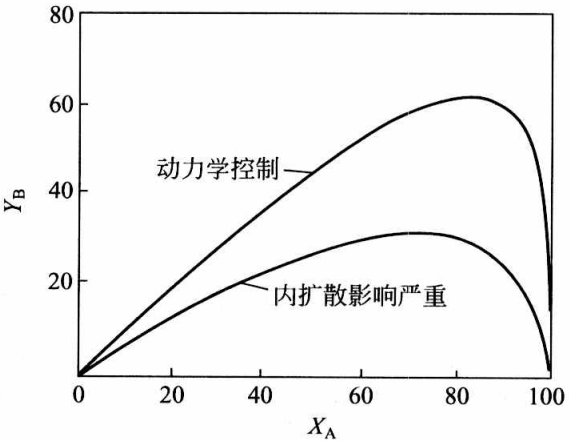
\includegraphics[width=\linewidth]{figures/fig6.7.png}
                \caption{内扩散对连串反应收率的影响}
            \end{figure}
        \end{minipage}

\end{frame}